Considera la expresión algebraica (\ref{eq:longitud_emb}) del Ejercicio \ref{ques:longitud_emb}.

\begin{multicols}{2}
    \begin{parts}

        Completa la tabla \ref{tab:longitud_emb}

        \begin{table}[H]
            \caption{Tabla con los datos de longitud y tiempo}
            \label{tab:longitud_emb}
            \begin{tabular}{|*{2}{p{2.5cm}|}}
                \toprule
                Tiempo de embarazo (semanas) & Longitud del feto (cm) \\\hline
                \midrule
                12                           &                        \\\hline
                                             & 13.19                  \\\hline
                14                           &                        \\\hline
                15                           &                        \\\hline
                                             & 17.78                  \\\hline
                17                           &                        \\\hline
                18                           &                        \\\hline
                                             & 22.37                  \\\hline
                20                           &                        \\\hline
                21                           &                        \\\hline
                22                           &                        \\\hline
                                             & 28.49                  \\\hline
                24                           &                        \\\hline
                25                           &                        \\\hline
                26                           &                        \\\hline
                27                           &                        \\\hline
                                             & 36.14                  \\\hline
                29                           &                        \\\hline
                30                           &                        \\\hline
                31                           &                        \\\hline
                32                           &                        \\\hline
                33                           &                        \\\hline
                                             & 45.32                  \\\hline
                35                           &                        \\\hline
                                             &                        \\\hline
                                             &                        \\\hline
                                             &                        \\\hline
                                             &                        \\\hline
                \bottomrule
            \end{tabular}
        \end{table}
        \columnbreak
        Grafica los datos en el plano cartesiano de la Figura \ref{fig:20230326214709}.

        \begin{figure}[H]
            \centering
            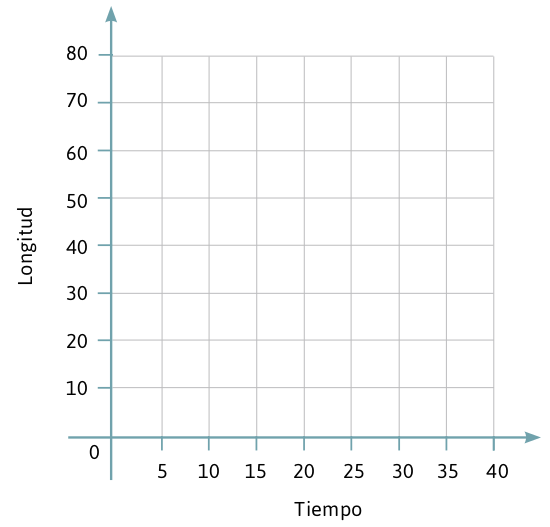
\includegraphics[width=0.45\textwidth]{../images/20230326214709}
            \caption{}
            \label{fig:20230326214709}
        \end{figure}

        Con base en la Tabla \ref{tab:longitud_emb}, ¿hay dos valores distintos de la variable $t$ que arrojen el mismo valor de $L$?

        \begin{solutionbox}{1.2cm}

        \end{solutionbox}

        Con base en la gráfica de la Figura \ref{fig:20230326214709}, ¿hay dos valores distintos de la variable $t$ que arrojen el mismo valor de $L$?

        \begin{solutionbox}{1.2cm}

        \end{solutionbox}

        ¿Hay algún valor de la longitud que proceda del valor 45 semanas?

        \begin{solutionbox}{1.2cm}

        \end{solutionbox}

        Y, ¿Hay algún valor de la longitud que proceda del valor 10 semanas? ¿Por qué?

        \begin{solutionbox}{1.2cm}

        \end{solutionbox}
    \end{parts}
\end{multicols}
